% Diagrama de lo que espera hacer mi algorimto con una caja negra que es un sistema automl. Esperar que el sistema se actualize solo!!!!!
% Escribir que es lo que espera mi algoritmo caja negra, y que es lo que retorna !!!!
% Escribir como si todo fuera desde yo, usando el imperseanl (No la primera persona)

\chapter{AutoML Heter\'ogeneo Multiobjetivo}\label{chapter:proposal}

AutoML Heter\'ogeneo Multibojetivo es una propuesta aplicable a cualquier sistema AutoML y permite resolver el problema definido en \ref{background:def:moo-automl-problem}. El n\'ucleo fundamental de la idea radica en trabajar sobre dos espacios bien definidos. El sistema busca y obtiene soluciones en el espacio de decisi\'on $\mathcal{X}$ y el resultado  de evaluar cada una de ellas se representa como un vector num\'erico donde cada una de sus componentes es la evaluaci\'on con respecto a cierta m\'etrica. Este vector representa un punto en el espacio objetivo $\mathcal{Y}$ con $\mathcal{Y} \subseteq \mathbb{R}^m$ donde $m$ representa el n\'umero de m\'etricas a evaluar. Cuando $m = 1$ es trivial saber cual es, basta encontrar el de mejor rendimiento. Cuando $m \ge 2$ ya no es tan f\'acil hablar del mejor pues pueden existir m\'as de uno; se habla en cambio de \textit{Pareto dominaci\'on} definido en (\ref{background:def:domintation}). La selecci\'on de los vectores  m\'as aptos del espacio de decisi\'on se realiza utilizando un algoritmo evolutivo multiobjetivo pues adem\'as de ser agn\'osticos al espacio de decisi\'on han demostrado ser los m\'as resistentes al frente de Pareto cuando tiene formas extra\~nas.

\section{Descripci\'on General}
\begin{figure}[ht]
    \centering
    %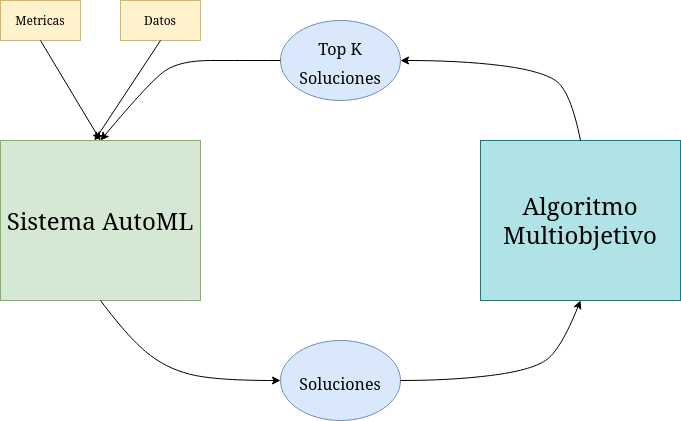
\includegraphics[scale=0.5]{Pictures/automl_moo_proposal.png}
    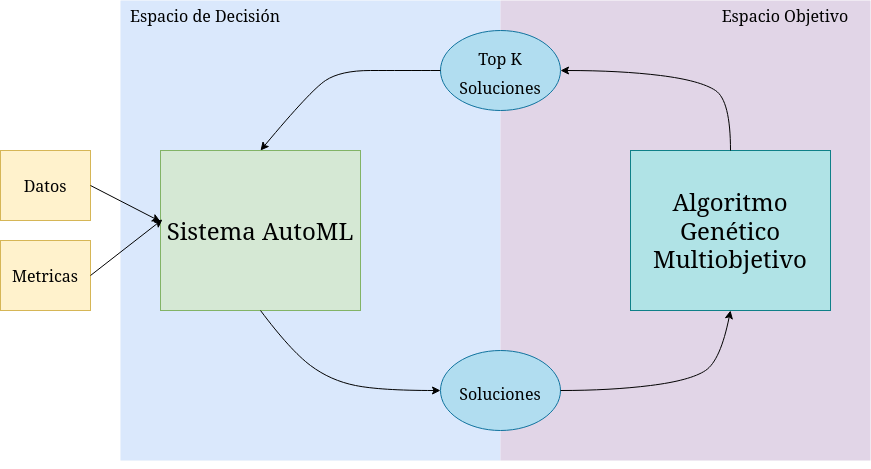
\includegraphics[scale=0.4]{Pictures/automl_moo_proposal2.png}
    \caption{Flujo general de la propuesta}
    \label{proposal:fig:flux}
\end{figure}

La soluci\'on propuesta (ver \ref{proposal:fig:flux}) est\'a compuesta por dos elementos fundamentales:
\begin{enumerate}
    \item Un sistema AutoML capaz de generar y evaluar m\'ultiples soluciones basado en un corpus de datos y un conjunto de m\'etricas. Las nuevas soluciones generadas deben poder tener en cuenta un conjunto de soluciones considerada las m\'as aptas. %m\'as aptas  partiendo de soluciones pasadas que se han considerado como las m\'as aptas;
    \item Un algoritmo de ordenaci\'on multiobjetivo capaz de funcionar solamente con el espacio objetivo y obtenga soluciones igualmente distribuidas a lo largo del frente de Pareto.
\end{enumerate}

La propuesta en cada iteraci\'on utiliza la evaluaci\'on de las soluciones generadas por el sistema de AutoML. La evaluaci\'on de una soluci\'on se representa como un vector $v$ de $m$ componentes donde $v_i$ es la evaluaci\'on de la soluci\'on con respecto a la m\'etrica $i$. El algoritmo ordena estos vectores utilizando alg\'un MOEA y retorna una lista ordenada de estos. Este proceso se repite hasta que se cumpla alg\'un criterio de parada.

% En su primera iteraci\'on el sistema AutoML debe producir una serie de soluciones y sus evaluaciones respectivas frente a las criterios de entrada. El algoritmo multiobjetivo debe ser capaz de ordenar efectivamente las soluciones de acuerdo a su evaluaci\'on tal que que los primeros $k$ elementos sean los m\'as aptos de para resolver el problema. Estas soluciones de mejor rendimiento se utilizan como entrada al sistema AutoML para que produzca una nueva generaci\'on de soluciones tomando la soluciones de entrada como referencia. El proceso se repite hasta que se cumpla el criterio de parada en donde se retornan los mejores individuos encontrados hasta el momento.

\subsection{Descripci\'on Formal}
El sistema propuesto est\'a compuesto por un sistema de Aprendizaje de M\'aquina Automatizado $\mathcal{A}(D, M, P)$  y un algoritmo evolutivo multiobjetivo $\mathcal{H}(TP)$. Los par\'ametros de entrada $D = \{(x_1, y_1), ..., (x_n, y_n)\}$ representa el conjunto de datos de entrada, $M = \{f_1, f_2, ..., f_m\}$ un conjunto de m\'etricas a evaluar, $P = \{p_1, p_2, ..., p_k\}$ el conjunto de soluciones de mejor rendimiento producidas por  $\mathcal{A}$ en la iteraci\'on anterior. $\mathcal{H}$ toma como entrada $TP$ que representa el conjunto de soluciones producidas en la iteraci\'on actual tras aplicar $\mathcal{A}(D, M, P)$. 
 %El objetivo final del sistema es producir una conjunto de soluciones de Aprendizaje Autom\'atico $P'$ que sean una muestra representativa del frente de Pareto (\ref{background:def:pareto_front}) utilizando un algoritmo multiobjetivo  $\mathcal{H}$ tal que $\mathcal{H}(TP) = P'$ en cierto n\'umero de iteraciones determinado por un criterio de parada. 
\begin{algorithm}[ht]\caption{Soluci\'on a AutoML Heter\'ogeneo Multiobjetivo}
    \KwIn{$\mathcal{A}$, D, M}
    \KwOut{P}
    $TP \gets \mathcal{A}(D, M, \emptyset)$ \tcp*{Se obtiene poblaci\'on inicial aleatoria}
    \While{no se cumplan condiciones de parada}{
        $P = \mathcal{H}(TP)$ \tcp*{Se extraen los m\'as aptos de una poblaci\'on} 
        $TP = \mathcal{A}(D, M, P)$ \tcp*{Se genera una nueva poblaci\'on}
    }
\end{algorithm}

La separaci\'on  por espacios existente entre ambas componentes de la propuesta permite generalizar el problema a cualquier tipo de sistema AutoML o funci\'on de ordenaci\'on. Todo sistema de AutoML que cumpla con estas condiciones es apto para la propuesta, no importa si est\'a enfocado en resolver el problema NAS o el problema CASH.
% Tambi\'en debe ser capaz de entender las carectr\'isticas que componen las soluciones m\'as aptas tal que en las subsecuentes iteraciones estas se conserven. Lograr esto \'ultimo requiere que el sistema tenga en cierta medida una implementaci\'on de algoritmos gen\'eticos para construir sus soluciones, por ende, la propuesta se adapta mejor a sistemas AutoML que utilizen programaci\'on evolutiva.

\section{MOEA}
%El algoritmo trabaja con vectores debido a que optimiza para varias m\'etricas, y no con un escalar que es trivial organizar. Como se meciona en \ref{background:def:moo} se hablar ahora de dominaci\'on y el adecuado ordenamiento es vital para escoger puntos del espacio que: (i) pertenzcan a los mejores frentes, (ii) que sean los elementos representativos del frente

Esencialmente cualquier tipo de ordenaci\'on para la que sea suficiente informaci\'on sobre espacio objetivo se puede utilizar. Especif\'icamente para esta propuesta utilizamos NSGA-II (\cite{deb2002fast}) por ser un algoritmo que sigue una idea intuitiva y tener un buen rendimiento general, suficiente para demostrar la efectividad de la propuesta.

\subsection{NSGA-II}
NSGA-II (\cite{deb2002fast}) es un algoritmo multiobjetvo basados en el frente de Pareto caracter\'isticos por dividir el proceso de ordenaci\'on en dos etapas (ver figura \ref{proposal:fig:nsga2}).

\begin{figure}[ht]
    \centering
    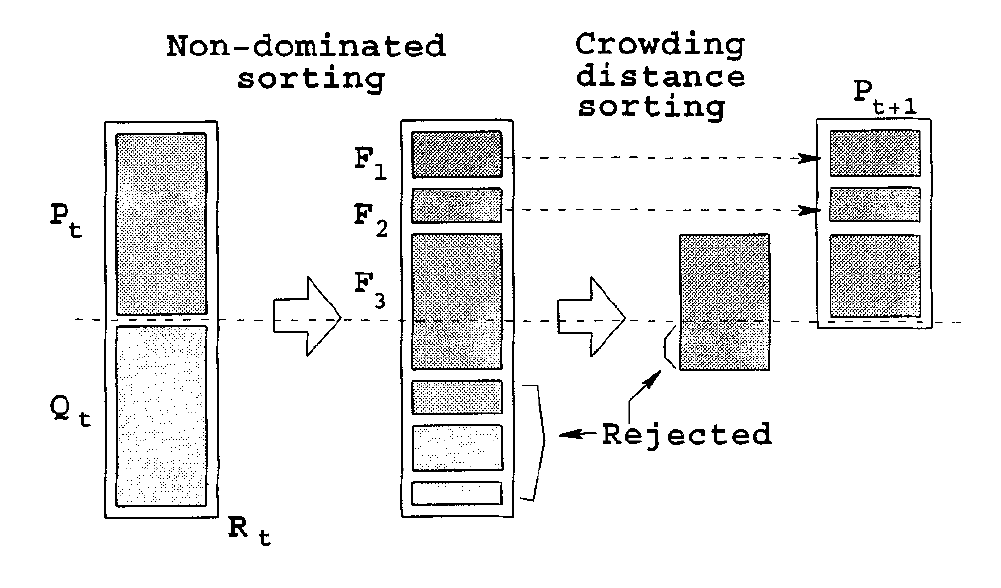
\includegraphics[scale=0.5]{Pictures/nsga2.png}
    \caption{Funcionamineto de NSGA-II}
    \label{proposal:fig:nsga2}
\end{figure}


La primera etapa llamada \textit{Non Dominated Sorting} agrupa las soluciones de acuerdo a su \'indice de dominaci\'on. El \'indice de dominaci\'on de una soluci\'on est\'a determinado por la cantidad de soluciones diferentes que la dominan.
\begin{definition}
    \label{proposal:def:domination_index}
    Dado un vector $x$ y un conjunto $Y$ de vectores en el espacio objetivo $\mathcal{Y}$ tal que los vectores en $Y$ dominan a $x$ (i.e. $Y = \{y | y \succ x\}$) se dice que $Ind(x) = |Y|$.
\end{definition}
\begin{definition}
    \label{proposal:def:rank_front}
    El conjunto de todas la soluciones con un mismo \'indice de dominaci\'on $i$ se les dice frente de rango $i$:
    \begin{equation*}
         F^i = \{x | x \in \mathcal{Y}, Ind(x) = i\}
    \end{equation*}
\end{definition}

El primer paso de \textit{Non Dominated Sorting} es calcular el \'indice de dominaci\'on de todas las soluciones. Revisa todos los pares de vectores $x, y \in \mathcal{Y}$ y calcula el \'indice  de cada uno mientras crea un grafo dirigido entre estos tal que existe una arista entre las soluciones $x$ y $y$ si $x \prec y$. Luego partiendo de las soluciones con \'indice de dominaci\'on 0, visita todas las soluciones que estas dominan y le reduce el \'indice de dominaci\'on en uno. El proceso se repite hasta que no queden soluciones por analizar.
El resultado de esta primera etapa es una lista ordenada  $F = \{F^0, ..., F^k\}$ de todos los frentes de distinto rango obtenidos. 
%$F^0$ contiene las mejores vectores a los cuales nadie domina e idealmente ser\'ia una aproximaci\'on al frente de Pareto.

%Es importante entender para la correctitud del aloritmo anterior  que las soluciones que conforman un frente de rango $i$ no se \textit{Pareto dominan} ($\prec$) entre si.
%Es f\'acilmente demostrable que la \texit{Pareto dominacion (i.e. $\prec$)} cumple con la propiedad de transitividad (i.e. si $x \prec y$, $y \prec z$, entonces $x \prec z$) 
%\begin{theorem}
%Dado $P^i$, frente de rango $i$, resultado de efectuar obtenido por Non Dominated Sort sobre una conjunto soluci\'on entonces $\neg \exists x, y \in P^i$ tal que $x \prec y$
%\end{theorem}
%% Definir correctamente la prueba
%Dado un frente de rango $i$ $F_i$, tal que existen soluciones $x, y \in F_i$ se asume que $x \prec y$. Como el \'inidice de dominaci\'on de $x$ es $i$ y $x \prec y$ y ($\prec$) es una operador transitivo entonces todos los que dominan a $x$ dominan a $y$, adem\'as del propio $x$, por tanto el inidice de dominaci\'on de $y$ ser\'ia $i+1$ lo que es una contradicci\'on porque $y \in F_i$. 

La segunda etapa llamada \textit{Crowding Distance Sorting} (CD),uno de los aportes claves hechos por \cite{deb2002fast}, ordena todos los frentes en $F$ con el objetivo de que los elementos con un ranking superior sean los elementos m\'as representativos del conjunto. Esta parte es vital pues permite en los casos donde haya que utilizar solo la porci\'on de un frente, se utilize la m\'as representativa de este. 
%En la segunda etapa los vectores de cada frente obtenido se organizan utilizando \textit{crowding distance} (CD), uno de las contribuciones claves de NSGA-II (\cite{deb2002fast}). El prop\'osito de \textit{crowding distance} es estimar la densidad de las soluciones con respecto sus soluciones vecinas de tal manera que los primeros lugares pertenezcan a los elementos m\'as representativos de dicho frente.

% Imagen de crowding distance
Calcular el CD de cada soluci\'on require ordenarlas seg\'un su valor normalizado por cada funci\'on objetivo y calcular el promedio de la distancia entre una soluci\'on y sus dos adyacentes respecto a dicha funci\'on objetivo. Esta distancia es el per\'imetro del cuboide formado usando los vecinos m\'as cercanos como v\'ertices. Los puntos que representan el m\'inimo y m\'aximo de al menos alguna funci\'on objetivo se les asigna \textit{crowiding distance} infinita. El  algoritmo queda descrito en \ref{proposal:alg:cd}.

\begin{algorithm*}[ht]
    \caption{Crowding Distance Sorting}
    \label{proposal:alg:cd}

    \tcp{F como entrada representa un frente de rango i}
    \KwIn{F} 
    \tcp{SF como salida representa el frente ordenado seg\'un CD}
    \KwOut{SF}
    \For{i desde 0 hasta $|F|$}{
        $F[i].dist \gets 0$ \;
    } 

    \ForEach{funcion objetivo $m$}{
        $F \gets ordenar(F, m)$ \tcp*{se ordena F con respecto a m}
        $F[0].dist \gets \infty$\;
        $F[|F|].dist \gets \infty$\;

        \For{i desde 2 hasta $|F| - 1$} {
            \begin{math}
                F[i].distance  = \frac{F[i].distance + (F[i + 1].m - F[i - 1].m)}{f^{max}_{m} - f^{min}_m}
            \end{math}
        }
    }
    $SF \gets ordenar(F, dist)$ \tcp*{se ordena F respecto a CD}
\end{algorithm*}


% Se obtiene como resultado un Grafo Aciclico Dirigido (DAG), donde cada arista representa una la expansi\'on de alg\'un no terminal de la gram\'atica. Un camino recorrido por dicho DAG es una posible soluci\'on de autogoal, referido como flujo o \textit{pipeline} de Aprendizaje Autom\'atico. A las aristas del DAG mantienen las probabilidades contenidas en $Prob$. Para recorrer cada camino se lanza utiliza una variable aleatoria uniforme y seg\'un su valor se escoge una producci\'on. Esto se realiza hasta obtener nuevas soluciones, hasta obtener una gran poblaci\'on.


% % Al inicio en el DAG las probabilidades est\'an igualmente distribuidas segu\'un el nodo y la cantidad de aristas (1 nodo con 3 aristas, 0.33 para cada uno) sobre todas las producciones por cada regla de la gram\'atica y se actualizan al aplicar PGE con el individuo m\'as apto donde se alterna entre aumentar ligeramente la probabilidad de las producciones que utilizadas por este y disminuir la probabilidades de los que no fueron utilizadas. Alternar entre estas dos v\'ias evita la utilizaci\'on del mismo individuo en iteraciones consecutivas balanceando la exploraci\'on global con explotaci\'on local.

% Como se trata de un problema multiobjetivo y no existe el individuo m\'as apto, sino un conjunto de estos las probabilidas se adaptan secuencialmente teniendo en cuenta cada uno de estos individuos.

 % (\textit{Probabilistic Grammatic Evolution}).
% En PGE se propone un cambio de como se interpreta el genotipo, ya no es una lista de enteros, sino u
% Utiliza Algirmtos de Estimacion de Distribucion (\textit{Estimation of Distribution Algorithms, EDA}) una t\'ecninca probabi\'istica que remplaza los operadores de mutaci\'on y cruce por un sampleando sobre la probabiliad de distribuci\'on de las producciones obtenidas por mejor individuo, para luego generar una nueva poblaci\'on por cada cada generaci\'on. Las probabilidades comienzan todas inicializadas en igual proporci\'on  y se actualizan basado en la frecuencia de las reglas de produccion escogidas para obtener el individuo con el mayor rendimiento.
% Probablisitic Grammatical Evolution (PGE)  se apoya en una Gramatica Probabilistica Libre del Contexto (\textit{Probilistic Context-Free Grammatic Evolution} PCFGE) para realizar los mapeos de los fenotipos a los genotipos. PCFGE se establece como una tupla $PG = (NT, T, S, P, Prob)$ donde $Prob$  es un conjunto de probabilidades asocaido con cada regla de la gram\'atica. El genotipo en PGE es un vector de numeros fraccionarios, donde cada uno corresponer con la probabiliad de seleccion cierta regla de derivaci\'on.
% insetar ejemplo de PGE.
% En PGE las probabilidades se actualizan despues de cada generaci\'on  despues de evaluar la poblaci\'on generada, basasdo en cuantas veces cada regla de derivacion fue seleccionada por el el individuo de mejor rendimiento. Si la regla fue seleccionada su probablidad incrementa, en cambio si no, su probabilidad se reduce. Alternando entre estas dos variantes se ayuda a evitar usar el mismo individuo en iteraciones consecutivas, balanceando exploracion global con expotacion local.
% \subsubsection{GE}
% Con esta idea en mente nace Grammatical Evolution, que utiliza una gramatica para establecer restricciones sint\'acticas sobre las soluciones individuales. Introudce la distinci\'on entre el genotipo y el fenotipo. 
% Para obtener una soluci\'on se tienen el genotipo (usualmente una lista de enteros) que se mapea al fenotipo (una lista de prdoucciones) siguiendo las reglas de producci\'on en una Gram\'atica Libre del Contexto (\textit{Context-Free Grammar}, CFG). Donde una gramatica es una terna $G = (NT, T, S, P)$ donde $NT$ y $T$ representan los conjuntos disjuntos no vac\'io de los s\'imbolos no terminales y terminales respectivamente. $S$ es un elemento de $NT$ llamado el axioma que representa el no-terminal principal que expandiendo este se puede llegar a todas las posibles formas de la gramatica. $P$ es el conjunto de reglas de producci\'on que rigen a la grma\'atica. Las reglas en $P$ tienen la forma de $A ::= \alpha$, donde $A \in NT$ y  $\alpha \in (NT \cup F)^*$ 
% Insertar ejemplo de como funciona esta talla
% El rendimiento de GE ha sido criticado en la literatura por tener alta redundancia y poca localidad. Una representaci\'on tiene alta redundancia cuando varios genotipos corresponden al mismo fenotipo y localidad se refiere a como los cambios en el genotipo se refeljean en el fenotipo. Con el objetivo de mejora GE han exisitido varias propuestas. Una de esta es Evoluci\'on de Gram\'atica Probabilistica.
